% Compile from this directory with build.ps1. Auxiliary files go to build/.
\RequirePackage{fix-cm}
\pdfminorversion=7
\newcommand{\DoNotLoadEpstopdf}{}
\documentclass[twocolumn]{svjour3}
\smartqed
\usepackage[utf8]{inputenc}
\usepackage{graphicx,microtype,hyperref}
\usepackage{amsmath,amssymb,amsfonts,booktabs,cite,array}
% Drop a PDF at the stated figures/ path to replace its placeholder automatically.
\newcommand{\paperfigure}[3]{%
  \IfFileExists{figures/#1}{%
    \includegraphics[width=\linewidth]{figures/#1}%
  }{%
    \fbox{\parbox[c][#2][c]{\dimexpr\linewidth-2\fboxsep-2\fboxrule\relax}{%
      \centering\small\textbf{Figure placeholder}\\[5pt]
      \texttt{\detokenize{#1}}\\[6pt]#3}}%
  }%
}
\newcommand{\draftnote}[1]{\par\smallskip\noindent\textit{Draft verification note: #1}\par\smallskip}

\begin{document}
\raggedbottom
\title{MobilePixorNeXt: Compact LiDAR Object Detection with Oriented Geometry and Localization Quality %\thanks{Grants or other notes The article that should go on the front page should be
%placed here. General acknowledgments should be placed at the end of the article.}
}
% \subtitle{Do you have a subtitle?\\ If so, write it here.

%\titlerunning{Short form of title}        % if too long for running head

\author{
        Duyen Huu Nguyen $^1$ \and
        Anh Duc Bui $^1$ \and
        Nhan Trong Phan $^1$ \and
        Hoang Ngoc Tran $^*$$^1$
        %etc.
}

%\authorrunning{Short form of author list} % if too long for running head

\institute{  *Correspondence: Hoang Ngoc Tran \\
 \at $^1$ 
              FPT University, Can Tho, 94000, VietNam. \\
%  \at $^2$ 
%               Department of Mechatronic Engineering, Faculty of Mechanical
%             Engineering, Ho Chi Minh City University of Technology (HCMUT),
% Vietnam National University, Ho Chi Minh City, Vietnam. \\
              \email{hoang2531992@gmail.com; duyennhce200017@gmail.com;  anhbdce200052@gmail.com; nhanptce200090@gmail.com}           %  \\
%             \emph{Present address:} of F. Author  %  if needed
}

\date{Received: date / Accepted: date}
%The correct dates will be entered by the editor

\titlerunning{MobilePixorNeXt}
\maketitle  


\begin{abstract}
Efficient LiDAR object detection requires a balance between geometric representation, feature processing, and the cost of producing final detections. We present MobilePIXORNeXt, a compact detector for oriented bird's-eye-view (BEV) footprints of cars, pedestrians, and cyclists. A deterministic fourteen-channel representation, Strata-BEV14, summarizes height, reflectance, density, occupancy, and within-cell point displacement. The narrow backbone applies SimAM within its residual blocks without adding attention parameters. Scale-gated fusion combines features at multiple resolutions. Grouped heads share an initial transformation across prediction tasks within each group. Training combines coordinate supervision, oriented geometric alignment, and a projection-based localization-quality target. The final architecture contains 753,569 detector parameters. The evaluation separates representation and component comparisons, geometric supervision, attention placement, and model-forward versus end-to-end latency. This separation provides a basis for assessing compact BEV detection without conflating network cost with complete-pipeline throughput.
% Add a quantitative performance conclusion only after the final protocol and
% conflicting workbook entries are reconciled against raw run reports.

\end{abstract}
\keywords{LiDAR detection \and Bird's-eye view \and Compact convolutional network \and SimAM \and Localization quality}

\section{Introduction}\label{sec:introduction}
\section{Introduction}
\IEEEPARstart{L}{iDAR} object detection supplies metric scene information for autonomous vehicles and mobile robots. The detector must recognize objects with different footprints and orientations from point clouds whose sampling varies with range and visibility. Bird's eye view (BEV) representations make this problem accessible to efficient two-dimensional convolutional networks. PIXOR established dense, proposal-free oriented detection from BEV inputs~\cite{yang2018pixor}, and PointPillars showed that learned pillar features can support fast detection with a two-dimensional backbone~\cite{lang2019pointpillars}. These approaches motivate a compact architecture that retains useful vertical statistics while allocating most learned processing to the horizontal plane.

Reducing parameter count leaves several design questions unresolved. A richer representation can preserve information discarded by a simple occupancy grid, but its benefit depends on the downstream model. Multi-scale context can strengthen feature processing, yet the resulting detections also depend on the regression objective and their ranking scores. A classification score alone does not explicitly encode localization quality. Conversely, a quality score learned from a footprint does not measure vertical overlap when the detector predicts full three-dimensional boxes. These relationships make component interactions relevant to the design of a small detector.

IRBGHR-PIXOR combines inverted residual blocks, Gaussian heatmap regression, and a modified focal objective for indoor pedestrian perception~\cite{nguyen2024indoor}. The present study addresses outdoor, three-class KITTI detection and develops a different architecture and geometric objective. Its Car, Pedestrian, and Cyclist results therefore answer a different evaluation question from IRBGHR-PIXOR's JRDB pedestrian results. We retain the useful connection between compact convolutions and Gaussian center supervision, while examining how geometry, quality estimation, and contextual refinement work together.

We introduce MobilePixorNeXt with a deterministic fourteen-channel representation, a convolutional hierarchy using $7\times7$ depthwise spatial mixing, scale-gated top-down fusion, and task groups for Car and Pedestrian/Cyclist. Oriented geometric alignment (OGA) combines a multi-axis projection objective with a footprint-scale-normalized corner distance and adaptive task weighting. A separate quality head, referred to as IQA in the implementation, predicts a detached geometric similarity and participates in detection scoring. We investigate these choices through an explicit $2\times2$ OGA--IQA comparison, matched OGA--Q-OGA retraining without a quality head, context and attention comparisons, checkpoint sensitivity, and runtime decomposition.

The study also evaluates a trained three-dimensional extension with shared head convolutions and a vertical regression branch. This extension provides a reference-evaluator result in addition to the local BEV ablation study. A conditional analysis of fixed BEV matches examines why adequate footprints can fail three-dimensional overlap thresholds. The principal contributions are the compact detector implementation, the observed interaction between geometric training and explicit quality prediction, and an evidence-based account of vertical localization limits. All reported runs use one random seed, and the numerical comparisons are confined to the protocols and training budgets under which they were obtained.

\begin{figure*}[t]
\centering
\includegraphics[width=.99\textwidth]{architecture_bev.pdf}
\caption{MobilePixorNeXt architecture used by the P16 BEV ablation. The fourteen-channel input produces a $32\times200\times176$ feature map through three convolutional stages, residual SimAM at stride four, focal context at stride eight, and scale-gated fusion. Car and Pedestrian/Cyclist have separate task groups with independent prediction branches. The trained Final3D extension shares the first head convolution within each group and adds a two-channel vertical branch; it is described in Section~\ref{sec:heads}. Dimensions omit the batch axis.}
\label{fig:architecture}
\end{figure*}

\section{Related Work}\label{sec:related_work}
\subsection{Bird's-Eye View LiDAR Representation and Pillar Encoding}
\label{sec:rel_bev_encoding}

Dense horizontal projection provides an efficient pathway to apply high-throughput 2D convolutional networks to unstructured 3D LiDAR point clouds. PIXOR~\cite{yang2018pixor} established the foundational paradigm of proposal-free Bird's-Eye View (BEV) detection by discretizing point clouds into fixed vertical occupancy slices and calibrated reflectance maps. Building upon this formulation, Nguyen et al.~\cite{nguyen2024indoor} introduced MobilePIXOR, replacing heavyweight convolutional layers with inverted residual blocks and Gaussian heatmap supervision for indoor robotic perception. In parallel, PointPillars~\cite{lang2019pointpillars} eliminated rigid vertical slicing by organizing point clouds into vertical columns (pillars) and learning spatial feature representations via localized PointNet encoders. Modern extensions such as PillarNeXt~\cite{li2023pillarnext} and PillarNeSt~\cite{mao2023pillarnest} systematically modernized pillar-based receptive field designs and backbone scaling for large-scale outdoor perception.

Despite their throughput advantages, existing BEV representations exhibit distinct structural trade-offs. On one hand, PointNet-based pillar encoders~\cite{lang2019pointpillars,li2023pillarnext} achieve expressive geometric learning, yet the non-deterministic point gathering, dynamic memory allocation, and sparse scatter operations incur prohibitive latency and energy penalties on edge accelerators. On the other hand, fixed-grid rasterization methods~\cite{yang2018pixor,nguyen2024indoor} bypass point gathering entirely but suffer from severe spatial quantization error on standard $0.1\,\text{m}$ grids; by treating cells as binary flags or raw counters, they discard critical continuous subcell offsets and high-order vertical distributions, causing boundary staircasing and localization jitter. While recent studies such as PillarHist~\cite{zhou2025pillarhist} investigate quantization-aware height histograms and TriBand-BEV~\cite{khoshkdahan2026triband} explores multi-band vertical slicing to assist pedestrian detection, a shared limitation across these paradigms is the absence of continuous subcell centroid displacements coupled with continuous vertical statistical moments inside a compact, hardware-friendly tensor. In summary, retaining fine continuous geometric boundaries without learned PointNet overhead remains an open research gap. MobilePIXORNeXt bridges this gap through the Strata-BEV14 representation (Section~\ref{sec:strata_bev14}). By deterministically integrating eight stratified vertical density bins, four continuous elevation moments ($\mu_z, \sigma_z, z_{\min}, z_{\max}$), and two continuous subcell centroid displacement offsets ($\Delta x_c, \Delta y_c$) into a 14-channel layout, Strata-BEV14 preserves sub-voxel geometric fidelity while reducing Host-to-Device transfer payloads by $60\%$ without learned encoder latency.

\subsection{Lightweight Convolutional Backbones and Efficient Spatial Attention}
\label{sec:rel_backbone_attention}

Extracting discriminative spatial semantics from sparse BEV feature planes requires balancing expressive receptive fields with strict parameter and latency constraints. In 3D LiDAR perception, volumetric detectors such as SECOND~\cite{yan2018second} popularized sparse convolutions to process non-empty voxels, while two-stage point architectures such as PointRCNN~\cite{shi2019pointrcnn} and hybrid frameworks such as Part-$A^2$~\cite{shi2020part} and PV-RCNN~\cite{shi2020pvrcnn} introduced part-aware aggregation and voxel-set abstractions. Although these methods achieve high detection accuracy on benchmarks such as KITTI~\cite{geiger2012kitti}, their multi-million parameter footprints ($4.0\text{--}63.8\,\text{M}$) and heavy memory access latencies ($130\text{--}195\,\text{ms}$) prohibit real-time deployment on power-constrained edge accelerators.

To overcome the latency bottleneck of volumetric processing, lightweight 2D convolutional designs have gained prominence. The ConvNeXt paradigm~\cite{liu2022convnext} demonstrated that conventional convolutions modernized with $7 \times 7$ depthwise kernels, inverted bottleneck expansions ($e=2.5$), and LayerScale can achieve representational power competitive with Vision Transformers while preserving convolutional hardware efficiency. Concurrently, lightweight attention mechanisms have been developed to emphasize salient geometric features. While Efficient Channel Attention (ECA-Net)~\cite{wang2020eca} captures 1D cross-channel interactions with low complexity, it lacks spatial feature modulation. To address this weakness, Yang et al.~\cite{yang2021simam} proposed SimAM, deriving full 3D spatial-channel attention weights analytically via an energy function inspired by visual neuroscience, requiring zero trainable parameters.

Collectively, a shared limitation of prior mobile LiDAR detectors is the reliance on standard inverted residual bottlenecks with small $3 \times 3$ kernels~\cite{nguyen2024indoor}, which struggle to capture multi-scale context across disparate vehicle and pedestrian dimensions. Furthermore, attempting to compensate by appending external attention modules or distillation schemes at coarse downsampling boundaries~\cite{tran2026rubber} introduces architectural overhead without resolving intra-block receptive field bottlenecks under sparse point distributions. In contrast, MobilePIXORNeXt incorporates the MobilePixorNeXt-S backbone with embedded parameter-free Block-SimAM (Sections~\ref{sec:backbone_architecture}--\ref{sec:next_s_block}) and a Top-Down Scale-Gated FPN (Section~\ref{sec:neck_architecture}), capturing expansive $7 \times 7$ depthwise receptive fields and modulating residual feature updates directly inside every residual block with zero added attention parameters.

\subsection{Geometric Supervision, Loss Formulations, and Quality Calibration}
\label{sec:rel_supervision_losses}

Bounding box regression in oriented object detection has progressively evolved from unconstrained coordinate offsets toward geometrically bounded objectives. Early detectors primarily relied on decoupled Smooth-L1 loss functions. However, regressing spatial coordinates, dimensions, and angles independently ignores the geometric interdependence of bounding boxes and induces severe gradient instability. To provide scale-invariant geometric feedback, Rezatofighi et al.~\cite{rezatofighi2019giou} introduced Generalized Intersection over Union (GIoU) to address gradient vanishing when candidate bounding boxes do not overlap. More recently, Le et al.~\cite{le2026mgiou} formulated Marginalized Generalized Intersection over Union (MGIoU), establishing a unified projection-based framework to optimize convex parametric shapes and arbitrary oriented bounding boxes without rotational singularities.

In parallel with geometric loss formulation, joint quality calibration has emerged as an essential mechanism for accurate detection ranking. Li et al.~\cite{li2020gfl} introduced Generalized Focal Loss (GFL), demonstrating that uncalibrated classification scores frequently disagree with actual localization quality, causing low-quality boxes with high confidence to suppress well-localized candidates during Non-Maximum Suppression (NMS). Additionally, Kendall et al.~\cite{kendall2018uncertainty} introduced multi-task uncertainty weighting, utilizing homoscedastic task variance to balance heterogeneous loss objectives across classification and geometric regression tasks.

Despite these advancements, existing oriented bounding box detectors still struggle with three pervasive limitations. First, independent angle and corner regression objectives remain susceptible to the $\pi$-periodicity boundary jump problem, where slight angular deviations around $\pm \pi/2$ or $\pm \pi$ trigger massive loss spikes and yaw gradient collapse. Second, conventional quality calibration mechanisms rely on auxiliary decoupled prediction heads that inflate model parameters and exacerbate gradient contention across heterogeneous object classes. Third, unconstrained multi-task uncertainty weighting allows task variance parameters to diverge, leading to training instability when balancing disparate loss scales across classification, geometric overlap, and orientation. Overall, developing a unified training formulation that simultaneously enforces orientation-symmetric geometric overlap, calibrated quality scoring (with or without dedicated heads), and bounded multi-task loss balancing remains an under-explored research gap. MobilePIXORNeXt bridges this gap through Oriented Geometric Alignment (OGA), its head-free alternative Q-OGA, and IoU-Aware Quality Alignment (IQA) (Section~\ref{sec:losses_and_oga}). Specifically, OGA unifies multi-axis MGIoU projections with scale-normalized $\pi$-symmetric corner supervision to eliminate boundary discontinuities; Q-OGA couples continuous IoU quality directly into classification supervision to achieve quality calibration with zero head overhead; IQA provides explicit multi-branch quality alignment scored via $S_{\mathrm{det}} = \sqrt{P_{\mathrm{cls}}\hat{q}}$ to suppress miscalibrated false positives; and Temperature-Softmax Bounded Uncertainty Weighting (T-SBUW) guarantees stable convergence by constraining multi-task weights within a normalized, bounded simplex.

\section{Proposed Method}\label{sec:method}
% Current method: user-confirmed F32, Tong hop last row 18 (2026-10-18).
% F24 historical hashes do not identify this F32 revision. See support/F32_REVISION_EVIDENCE.md.
% Paper name Strata-BEV14 maps to the unchanged hist14 v1 checkpoint encoding.

MobilePIXORNeXt maps a LiDAR scan to class-labelled oriented BEV boxes through deterministic feature encoding, a compact convolutional hierarchy, multiscale fusion, and grouped prediction heads. Figure~\ref{fig:r37_overview} summarizes the configuration used as the main detector, denoted R37-F32 here to distinguish it from the earlier F24 run. Its outputs describe horizontal location, footprint dimensions, orientation, and localization quality. Vertical box coordinates are not predicted by this configuration; any separately trained 3D extension is evaluated as a distinct variant.

\begin{figure*}[t]
    \centering
    \paperfigure{pipeline_overview.pdf}{30mm}{Source: slide PDF page 1; complete overview page, preserving vector labels and embedded point-cloud images.}
    \caption{Overview of MobilePIXORNeXt. Strata-BEV14 converts the scan into a fixed statistical grid; the detector predicts class heatmaps, center offsets, footprint dimensions, doubled yaw, and localization quality. The main model predicts oriented BEV footprints, shown over the 3D input cloud. The dashed feedback path is used only in training. FL denotes Gaussian focal classification, BCE supervises localization quality, and T-SBUW denotes the adaptive task balancing described in the text.}
    \label{fig:r37_overview}
\end{figure*}


\subsection{Strata-BEV14 point-cloud encoding}
\label{sec:rich_bev14}

The representation is inspired by the height-stratified BEV design of TriBand-BEV~\cite{khoshkdahan2026triband}, whose three channels store band-wise maximum corrected reflectance. We retain the idea of summarizing vertical structure on a horizontal grid, but use different band definitions and statistical channels. We call the two configurations Strata-BEV8 and Strata-BEV14; their suffixes denote channel counts, not height-band counts. These names describe our configured encodings, rather than a reproduction of TriBand-BEV.

Height histograms provide another source of inspiration~\cite{zhou2025pillarhist}. We use four log-scaled count bins, cell statistics, and mean subcell offsets. The resulting fourteen-channel raster is deterministic; it does not reproduce the learned pillar encoder in that work or establish its reported quantization benefits for our detector.

A scan is represented by $\mathcal P=\{(x_i,y_i,z_i,\iota_i)\}_{i=1}^{N_{\mathrm{pts}}}$, where $\iota_i$ is reflectance. The LiDAR frame uses forward $x$, leftward $y$, and upward $z$. We retain finite points within the region $[0,70.4]\times[-40,40]\times[-2.5,1.0]$~m, applying strict bounds with a $0.001$~m inward margin. A horizontal resolution of $\Delta_x=\Delta_y=0.1$~m produces $800\times704$ cells. Point assignment uses
\begin{equation}
    u_{\mathrm{in}}=\left\lfloor\frac{x_i-x_{\min}}{\Delta_x}\right\rfloor,
    \qquad
    v_{\mathrm{in}}=\left\lfloor\frac{y_i-y_{\min}}{\Delta_y}\right\rfloor.
    \label{eq:input_grid}
\end{equation}

Strata-BEV14 encodes each occupied cell using the fourteen statistics in Table~\ref{tab:rich_bev14}. Heights are normalized as $\zeta_i=(z_i-z_{\min})/(z_{\max}-z_{\min})$, and reflectance is clipped to $[0,1]$. Four equal-height intervals summarize the vertical distribution. Their count channels and the total-density channel use
\begin{equation}
    d_{\log}(N)=\min\left(1,\frac{\log(1+N)}{\log(33)}\right),
    \label{eq:density_encoding}
\end{equation}
where $N$ is the corresponding cell or bin count. These channels are density statistics rather than histogram probabilities. The remaining statistics describe height variation, reflectance, occupancy, and subcell point locations. Empty cells are zero, and the resulting input is $\mathbf X\in\mathbb R^{B\times14\times800\times704}$.

\begin{table}[t]
    \caption{Strata-BEV14 channels, indexed from zero. All statistics are computed over points in one input cell.}
    \label{tab:rich_bev14}
    \centering\small
    \begin{tabular}{@{}p{0.15\columnwidth}p{0.77\columnwidth}@{}}
        \toprule
        Channels & Cell statistics \\
        \midrule
        0--3 & Log-normalized counts in four equal-height intervals. \\
        4--7 & Maximum, mean, span, and population standard deviation of $\zeta_i$. \\
        8--9 & Maximum and mean clipped reflectance. \\
        10--11 & Log-normalized total count and binary occupancy. \\
        12--13 & Mean point displacement from the input-cell center, divided by $\Delta_x$ or $\Delta_y$ and clipped to $[-0.5,0.5]$. \\
        \bottomrule
    \end{tabular}
\end{table}

This deterministic encoding retains vertical summaries while allowing the learned network to operate entirely on a horizontal grid. The normalized point displacements describe the distribution of observations within an input cell; they are distinct from the metric object-center offsets predicted by the detector.

Strata-BEV8 starts with three occupancy channels for equal-height bands. These are followed by maximum and mean normalized height, maximum and mean clipped reflectance, and total log-density. Its occupancy bands indicate whether a return exists; they do not store band-wise reflectance. Strata-BEV14 changes the vertical summary to four log-count bands and adds height span, height standard deviation, whole-cell occupancy and mean subcell offsets. Consequently, the eight-channel encoding is not simply a subset of the fourteen-channel tensor. Both use the configured sensor-frame height interval; neither applies TriBand-BEV's ground-referenced band thresholds or reflectance offset and gain. The implementation keys remain \texttt{rich8} and \texttt{hist14} (v1) for reproducibility.

\subsection{Compact convolutional hierarchy}
\label{sec:method_backbone}

The stem contains two $3\times3$ convolutions with 32 output channels and strides two and one, respectively. Each is followed by batch normalization (BN) and SiLU. Three subsequent stages begin with a stride-two $3\times3$ convolution and contain 3, 4, and 2 residual blocks. Their outputs have 48, 96, and 128 channels at strides 4, 8, and 16. We index features by their spatial stride, $\mathbf F^{(r)}$, to make the resolution of each connection explicit.

Figure~\ref{fig:backbone} specifies the feature hierarchy and shared grouped heads. The final fusion width is 32 channels; it should not be confused with the earlier F24 configuration carrying the same workbook identifier.

\begin{figure*}[t]
    \centering
    \paperfigure{backbone_f32.pdf}{44mm}{Source: current slide PDF page 3; residual block on page 4 and fusion on page 5.}
    \caption{Final backbone, fusion neck, and prediction heads. Spatial strides are 2 at the stem and 4, 8, and 16 at the three subsequent stages. Lateral widths are 32, 48, and 48, and the final shared feature has shape $32\times200\times176$. Prediction maps have 176 columns; the Pedestrian/Cyclist heatmap has two channels. Stages are identified here by strides 4/8/16; the drawing retains legacy C2/C3/C4 labels, and its deepest stage label refers to the stride-16 stage. Each group uses a shared $3\times3$--BN--SiLU stem; each private Conv box abbreviates $3\times3$--BN--SiLU followed by a $1\times1$ output projection.}
    \label{fig:backbone}
\end{figure*}

The residual block adopts large-kernel depthwise spatial mixing and inverted channel expansion, following modern convolutional design principles~\cite{liu2022convnext}. For a $C$-channel input $\mathbf Z$, its transformation is
\begin{align}
    \mathbf V &= \operatorname{BN}(\operatorname{DWConv}_{7\times7}(\mathbf Z)),\nonumber\\
    \mathbf R &= \operatorname{BN}\!\left(W_{\mathrm{red}}\,
        \operatorname{SiLU}(W_{\mathrm{exp}}\mathbf V)\right),\nonumber\\
    \mathbf Z' &= \mathbf Z+\boldsymbol\gamma_{\mathrm{blk}}\odot\mathcal S(\mathbf R).
    \label{eq:next_block}
\end{align}
Here $W_{\mathrm{exp}}$ and $W_{\mathrm{red}}$ are $1\times1$ convolutions that expand channels from $C$ to $2.5C$ and project them back to $C$. The operator $\mathcal S$ denotes block-level SimAM, defined below. The learned channel-wise residual scale $\boldsymbol\gamma_{\mathrm{blk}}$ is initialized to $10^{-5}$. The final model uses ordinary depthwise convolutions without structural reparameterization or an additional detail branch.

\subsection{Block-level SimAM refinement}
\label{sec:method_refinement}

The final model applies SimAM~\cite{yang2021simam} inside every residual block of the three backbone stages, corresponding to C3, C4, and C5 at strides 4, 8, and 16. With stage depths $(3,4,2)$, the backbone contains nine SimAM operators. Each operator acts on $\mathbf R$, the output of the channel-reduction convolution and its BN, before the existing LayerScale and shortcut addition in Eq.~\ref{eq:next_block}. Figure~\ref{fig:r37_refinement} shows this ordering. Thus, attention changes the residual update while leaving the identity shortcut intact.

For a residual tensor $\mathbf R\in\mathbb R^{B\times C\times H\times W}$, let $\mu_c^{\mathrm{sp}}$ be the spatial mean within channel $c$ and define
\begin{equation}
    \nu_c^{\mathrm{sp}}=\frac{\sum_{v,u}(R_{cvu}-\mu_c^{\mathrm{sp}})^2}{\max(HW-1,1)}.
    \label{eq:simam_variance}
\end{equation}
The batch index is omitted; statistics are computed independently for each example and channel. The elementwise gate and attended update are
\begin{align}
    A_{cvu} &= \sigma\!\left(
        \frac{(R_{cvu}-\mu_c^{\mathrm{sp}})^2}
        {4(\nu_c^{\mathrm{sp}}+\lambda_{\mathrm{sim}})}+\frac12\right),\nonumber\\
    \mathcal S(\mathbf R) &= \mathbf A\odot\mathbf R,
    \label{eq:block_simam}
\end{align}
with $\lambda_{\mathrm{sim}}=10^{-4}$. The gate assigns larger weights to activations whose squared deviation from the channel mean is larger relative to its spatial variance. This operation uses feature statistics rather than point occupancy or learned query--key interactions. Spatial moments and gate values are computed in FP32, then the gate is cast to the feature dtype for multiplication.

SimAM introduces no learned parameters in this placement. The existing channel-wise scale $\boldsymbol\gamma_{\mathrm{blk}}$ controls the attended residual; there is no additional scalar wrapper. This differs from applying a residual attention adapter after an entire stage. The final model enables block attention at all three stages, with no separate stage-level attention or focal-context module.

\begin{figure*}[t]
    \centering
    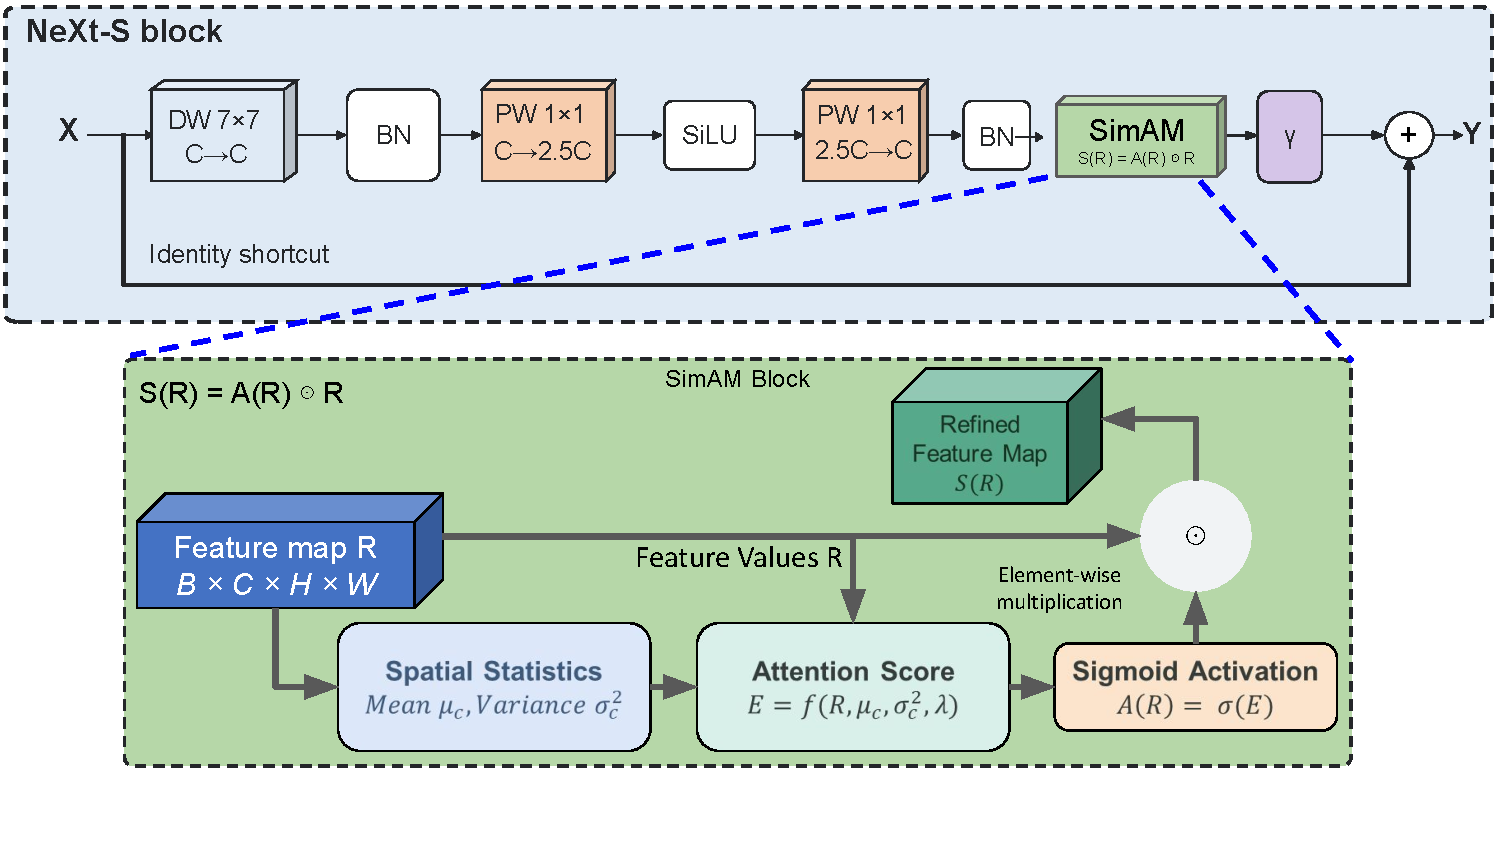
\includegraphics[width=\textwidth]{figures/next_simam_block.pdf}\\[6pt]
    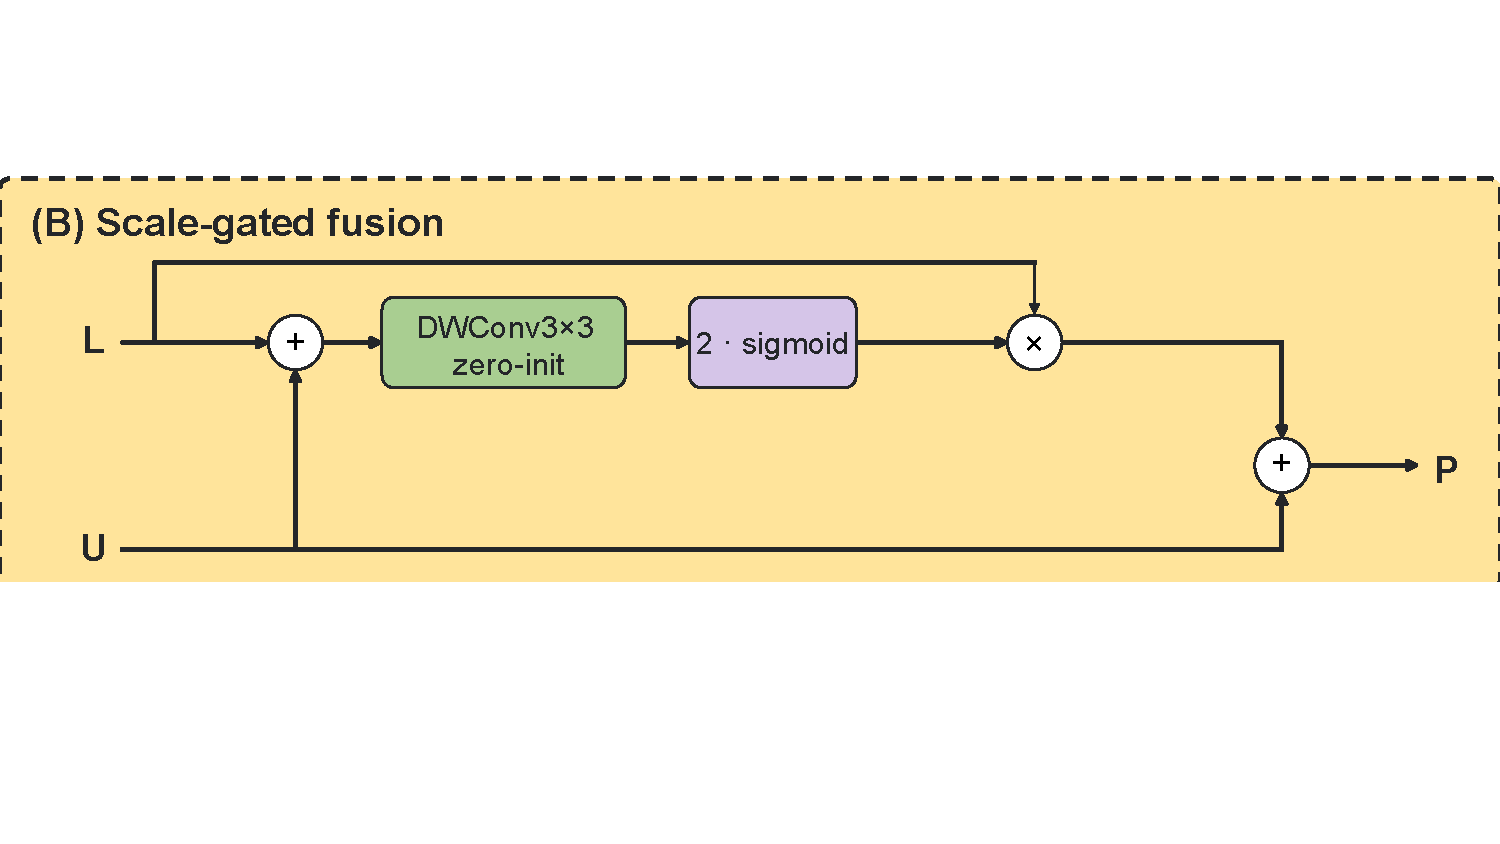
\includegraphics[width=0.70\textwidth]{figures/scale_gated_fusion.pdf}
    \caption{Two building blocks extracted as vector graphics from the authors' slide export. (A) NeXt residual block with SimAM after projection BN and before LayerScale. The SimAM operator acts on the intermediate residual tensor $\mathbf R$ in Eq.~\ref{eq:next_block}, consistently labeled R in the drawing. (B) Scale-gated fusion of lateral feature $\mathbf L$ and top-down feature $\mathbf U$, yielding $\mathbf P$. Addition and elementwise multiplication are shown explicitly.}
    \label{fig:r37_refinement}
\end{figure*}


\subsection{Scale-gated multiscale fusion}
\label{sec:method_neck}

The neck projects the stride-16 and stride-8 features to 48 channels, and the stride-4 feature to 32 channels. At stride eight, bilinear upsampling of the deepest lateral feature is followed by a depthwise $3\times3$ convolution, BN, and SiLU. The resulting top-down feature $\mathbf U_8$ is fused with lateral feature $\mathbf L_8$. A second bilinear upsampling and a standard $3\times3$ projection from 48 to 32 channels produce $\mathbf U_4$ for fusion with $\mathbf L_4$. Interpolation uses \texttt{align\_corners=False}.

Figure~\ref{fig:r37_refinement}(B) illustrates the fusion operator. At each fusion stride $r\in\{4,8\}$,
\begin{align}
    \mathbf G_r &= 2\sigma\!\left(
        \operatorname{DWConv}_{3\times3,r}(\mathbf L_r+\mathbf U_r)\right),\nonumber\\
    \mathbf P^{(r)} &= \mathbf U_r+\mathbf G_r\odot\mathbf L_r.
    \label{eq:scale_gated_fusion}
\end{align}
Gate weights and biases are zero-initialized, so fusion initially reduces to addition. A final $3\times3$ convolution from 32 to 32 channels, BN, and SiLU produce the shared detector feature $\mathbf F_{\mathrm{out}}\in\mathbb R^{B\times32\times200\times176}$. The gate can adjust each lateral response using information from both paths without replacing the top-down feature.

\subsection{Grouped prediction and target assignment}
\label{sec:method_heads}

The first task group contains Car ($K_1=1$), and the second contains Pedestrian and Cyclist ($K_2=2$). Each group first applies a shared $3\times3$ convolution with 32 channels, BN, and SiLU. Its output feeds five branches for classification, center offset, log-size, doubled yaw, and quality. Each branch contains one private $3\times3$ convolution with 32 channels, BN, and SiLU, followed by a $1\times1$ output convolution. Each prediction path therefore still traverses two $3\times3$ convolutions, while its first transformation is shared across tasks. The two groups own separate shared convolutions and branch weights. Geometry and quality maps are shared across the classes within a group.

For a group with $K_g$ classes, the output channel counts are $(K_g,2,2,2,1)$. At output location $(u,v)$, the geometric targets are
\begin{align}
    \mathbf o^* &= \begin{pmatrix}
        x^*-x_{\min}-u s_{\mathrm{out}}\Delta_x\\
        y^*-y_{\min}-v s_{\mathrm{out}}\Delta_y
    \end{pmatrix},\nonumber\\
    \mathbf d^* &= (\log w^*,\log l^*),\qquad
    \mathbf a^*=(\cos2\psi^*,\sin2\psi^*),
    \label{eq:regression_targets}
\end{align}
where $s_{\mathrm{out}}=4$ and sizes inside logarithms are expressed numerically in metres. The doubled angle represents footprint orientation modulo $\pi$.

Classification uses class-specific Gaussian heatmaps with peaks at quantized object centers. The radius is determined from the footprint dimensions in output cells using overlap setting 0.1 and a minimum radius of four cells. Regression supervision occupies a disk with half that heatmap radius. Where disks overlap, cells are assigned to the nearest continuous object center, with quantized center cells reserved for their owning targets. This produces a single valid regression target per group and location, indicated by $\mathbf M_{\mathrm{reg}}$.

\subsection{Oriented geometry and quality supervision}
\label{sec:method_objective}

The OGA objective combines classification, coordinate regression, footprint geometry, and quality prediction. Classification uses the Gaussian focal form: unit-valued heatmap peaks have modulating factor $(1-p_{\mathrm{cls}})^2$, while other cells use $p_{\mathrm{cls}}^2(1-Y^*)^4$. The summed loss is normalized by the number of positive peaks; an image batch without peaks retains the negative sum. Offset, log-size, and doubled-yaw losses use Smooth-L1 with transition parameter one, averaged over the valid regression elements. Numerical normalization adds $10^{-4}$ to the element count.

For each valid regression cell, predicted and target footprints are decoded into four corners. Following Marginalized Generalized Intersection over Union (MGIoU)~\cite{le2026mgiou}, both rectangles are projected onto the length and width axes of the prediction and target. On each axis, we compute one-dimensional Generalized Intersection over Union (GIoU)~\cite{rezatofighi2019giou}. For projection axis $k$, let $I_k$, $U_k$, and $E_k$ be the intersection, union, and enclosing interval lengths. Define
\begin{align}
    g_k &= \frac{I_k}{U_k}-\frac{E_k-U_k}{E_k},\nonumber\\
    \bar g &= \frac14\sum_{k=1}^{4}g_k,\qquad
    \ell_{\mathrm{proj}}=\frac{1-\bar g}{2}.
    \label{eq:projected_geometry}
\end{align}
Here $\bar g$ is the rectangle-specific MGIoU similarity and $\ell_{\mathrm{proj}}$ is its normalized loss. Denominators are floored at $10^{-6}$. This compares one-dimensional projections rather than computing polygon intersection area.

The corner term measures average L1 corner discrepancy under two equivalent correspondences. Let $\widehat{\mathbf c}_m$ and $\mathbf c_m^*$ denote ordered footprint corners, and let $\Pi_\pi$ contain the identity and the permutation induced by a $\pi$ rotation. Then
\begin{equation}
    \ell_{\mathrm{corner}}=
    \frac{\displaystyle\min_{\pi\in\Pi_\pi}\frac14
        \sum_{m=1}^{4}\|\widehat{\mathbf c}_m-\mathbf c_{\pi(m)}^*\|_1}
    {\max\!\left(\sqrt{(w^*)^2+(l^*)^2},10^{-6}\right)}.
    \label{eq:symmetric_corners}
\end{equation}
Target-diagonal normalization scales the discrepancy relative to object size, and the two correspondences respect the doubled-angle representation. The geometry objective is the mean of $\ell_{\mathrm{proj}}+\beta_{\mathrm{corner}}\ell_{\mathrm{corner}}$ over valid cells, with $\beta_{\mathrm{corner}}=1$. Geometry calculations use FP32, clamp log-dimensions to $[-10,10]$, and use zero yaw when the doubled-angle vector norm is below $10^{-6}$.

The IQA branch predicts $\hat q=\sigma(\hat Z_{\mathrm{qual}})$ and is supervised at valid regression cells using binary cross-entropy. Its target is
\begin{equation}
    q_{\mathrm{proj}}^*=\operatorname{stopgrad}
        \bigl(\operatorname{clip}(\bar g,0,1)\bigr).
    \label{eq:quality_target}
\end{equation}
The target uses the clipped MGIoU similarity, not the geometry loss. It is detached from box decoding, so this supervision does not backpropagate through the target geometry. Although the implementation names the branch IoU-aware quality, the final model learns a projection-based similarity, not exact BEV or 3D IoU. Its coefficient before adaptive balancing is one.

\subsection{Adaptive task balancing}
\label{sec:method_balance}

Each group independently balances six loss terms, indexed by $\mathcal T=\{\mathrm{cls},\mathrm{off},\mathrm{size},\mathrm{yaw},\mathrm{geo},\mathrm{qual}\}$ with $J=6$. Learned logits $a_k$ determine positive weights through a bounded temperature softmax:
\begin{align}
    \bar a_k &= b_{\mathrm{uw}}\tanh(a_k/b_{\mathrm{uw}}),\nonumber\\
    \omega_k &= J\frac{\exp(\bar a_k/\tau_{\mathrm{uw}})}
        {\sum_{j\in\mathcal T}\exp(\bar a_j/\tau_{\mathrm{uw}})},
    \label{eq:task_weights}
\end{align}
where $b_{\mathrm{uw}}=3$ and $\tau_{\mathrm{uw}}=2$. Zero-initialized logits give unit initial weights. An exponential moving average $\mu_k$ tracks the detached, floored task loss with momentum $\beta_{\mathrm{EMA}}=0.99$, initialized from the first training batch. For group $g$, the balanced objective is
\begin{equation}
    \mathcal L_g=\left(\frac1J\sum_{k\in\mathcal T}\mu_k\right)
        \sum_{k\in\mathcal T}\omega_k
        \frac{\mathcal L_k}{\max(\mu_k,10^{-4})}.
    \label{eq:balanced_objective}
\end{equation}
The full loss is $\mathcal L_{\mathrm{total}}=0.5\mathcal L_1+0.5\mathcal L_2$. Running-scale normalization compensates for differences in task-loss magnitude before weighting. These adaptive weights are optimization variables, not calibrated estimates of statistical uncertainty. The two groups introduce twelve training-only logits, separate from the detector parameters used at inference.

\subsection{Decoding and inference}
\label{sec:method_decode}

Predicted offsets are in metres relative to output-grid origins. Box decoding is
\begin{align}
    \hat x &= x_{\min}+u s_{\mathrm{out}}\Delta_x+\hat o_x,\nonumber\\
    \hat y &= y_{\min}+v s_{\mathrm{out}}\Delta_y+\hat o_y,\nonumber\\
    \hat w &= \exp(\hat d_1),\qquad \hat l=\exp(\hat d_2),\nonumber\\
    \hat\psi &= \tfrac12\operatorname{atan2}(\hat a_2,\hat a_1).
    \label{eq:box_decode}
\end{align}
No half-cell shift is added. Classification and quality predictions are combined as
\begin{equation}
    s_{\mathrm{det}}=p_{\mathrm{cls}}^{1-\alpha_{\mathrm{score}}}
        \hat q^{\alpha_{\mathrm{score}}},\qquad \alpha_{\mathrm{score}}=0.5.
    \label{eq:quality_ranking}
\end{equation}
Candidates are selected from $3\times3$ local maxima of this ranking score independently for each class. Both $p_{\mathrm{cls}}$ and $s_{\mathrm{det}}$ must exceed 0.05. Classwise rotated BEV non-maximum suppression uses an IoU threshold of 0.1, followed by a global limit of 500 detections per scan. These decoding thresholds are separate from the overlap thresholds used to evaluate detection accuracy.

The complete F32 detector has 753,569 learned parameters, excluding the adaptive loss weights. The selected workbook configuration uses hybrid ground-truth sampling. Section~\ref{sec:experiments} distinguishes the verified model specification from training and timing settings still requiring the final run records.

\section{Experiments}\label{sec:experiments}
\subsection{Dataset and reporting protocol}

The study considers the Car, Pedestrian, and Cyclist classes in KITTI~\cite{geiger2012kitti}. The repository split manifests contain 3,712 training and 3,769 validation frames. The final run must be linked to these exact manifests before the split is treated as its verified training record. All primary detection tables in this draft concern BEV footprints; the model does not regress vertical position or height.

We use the class-specific overlap thresholds $\tau_{\mathrm{IoU},c}=0.70$ for Car and $0.50$ for Pedestrian and Cyclist. At a fixed difficulty, Moderate macro mAP is the unweighted mean across the three classes. The secondary quantity mAP9 averages the nine class--difficulty combinations:
\begin{align}
    \mathrm{mAP}_{\mathrm M} &= \frac{1}{3}\sum_{c\in\mathcal C}\mathrm{AP}_{c,\mathrm M},\nonumber\\
    \mathrm{mAP}_{9} &= \frac{1}{9}\sum_{c\in\mathcal C}
    \sum_{d\in\{\mathrm E,\mathrm M,\mathrm H\}}\mathrm{AP}_{c,d}.
    \label{eq:map_definitions}
\end{align}
The symbols E, M, and H denote Easy, Moderate, and Hard. AP and both aggregates are expressed as percentages. mAP9 is not AP at IoU 0.9.

Historical local BEV evaluation and reference KITTI evaluation have different ground-truth domains and matching rules. Consequently, the ablation summary and detector-comparison summary are maintained as distinct experiment sets. The intended AP sampling is R40, but the evaluator version, split, sampling and filtering rules must be recovered for each final comparison record before it is presented as a matched benchmark.

\begin{table}[t]
\centering\small
\caption{Verified model settings and remaining run-specific fields.}
\label{tab:setup}
\begin{tabular}{@{}>{\raggedright\arraybackslash}p{.38\columnwidth}>{\raggedright\arraybackslash}p{.55\columnwidth}@{}}
\toprule
Setting & Value \\
\midrule
Input & Strata-BEV14; $14\times800\times704$ \\
ROI (m) & $x:[0,70.4]$; $y:[-40,40]$; $z:[-2.5,1]$ \\
XY cell / output stride & 0.1 m / 4 \\
Stage widths / depths & 48, 96, 128 / 3, 4, 2 \\
Fusion / Head width & 32 / 32 \\
Prediction groups & Car; Pedestrian + Cyclist \\
Training objective & OGA + projection-target IQA \\
Sampling recipe & PC-GTA \\
Final run / checkpoint & Pending resolved config and hash \\
Training schedule / seeds & Pending final run record \\
AP protocol / split hashes & Pending per experiment set \\
Hardware / timing setup & Pending per benchmark record \\
\bottomrule
\end{tabular}
\end{table}


\subsection{Model and training configuration}

The selected configuration uses Strata-BEV14, nine block-level SimAM operators, F32 scale-gated fusion, grouped shared H32 heads, OGA, and a separate IQA branch. The final-width decision was made after the earlier F24 run; reusing the shorthand R37 does not imply that the two configurations share a checkpoint. The current architecture contains 753,569 detector parameters and twelve additional training-only task-balancing logits. The parameter count is obtained directly from model construction and excludes optimizer state and running buffers.

Hybrid ground-truth sampling is selected in the current experiment summary. The final optimizer, schedule, physical batch size, accumulation, augmentation probabilities, checkpoint-selection rule and precision are reserved for the resolved training record. Earlier configurations contain plausible defaults, but those defaults are not substituted for the final run's provenance. Table~\ref{tab:setup} records the remaining fields explicitly.

\subsection{Comparison design}

The evaluation is organized around three questions. First, a sequence of configuration comparisons examines the backbone, BEV representation, grouped prediction, sampling strategy, fusion width, and neck. This sequence describes the development of a complete recipe; a transition supports a single-factor interpretation only when its other settings are matched. Second, a factorial comparison separates baseline/OGA supervision from the presence of IQA. Q-OGA is treated as an additional objective rather than another cell of the same factorial design. Third, attention comparisons distinguish stage-level SimAM from SimAM within each residual block, while recording fusion width and head sharing.

For the OGA--IQA experiment, an interaction in mAP can be summarized as
\begin{equation}
    \Delta_{\mathrm{int}}=m_{11}-m_{10}-m_{01}+m_{00},
    \label{eq:interaction}
\end{equation}
where the first index denotes OGA and the second denotes IQA. This quantity is meaningful only for matched runs with a consistent baseline; it is not computed from the conflicting baseline records in the current workbook.

\subsection{Complexity and timing}

Forward timing starts with prepared inputs already on the device. End-to-end latency covers the measured input-to-detections pipeline, whose inclusion of file loading, encoding, transfers, decoding, and NMS must be specified by the benchmark record. For sequential batch-one processing, reciprocal-mean throughput is $1000/\bar t$ FPS when mean latency $\bar t$ is in milliseconds. This is distinct from averaging per-frame reciprocal latency.

Forward latency, end-to-end latency and their percentiles are reported separately. Stage percentiles are not summed to obtain a pipeline percentile. A matched runtime comparison requires the same hardware, precision, batch size, warmup, timed frames and timing boundaries. The revised summary contains no verified FLOP/MAC or memory measurements, so those quantities remain unreported rather than inferred from parameter count. Repeated training seeds and timing sessions are also needed before reporting uncertainty or statistical significance.

\section{Results and Discussion}\label{sec:results}
\subsection{Quantitative Comparison on KITTI Benchmark}
\label{sec:benchmark_comparison}

\begin{table*}[t]
\centering\small
\caption{Multi-seed statistical robustness and variance comparison between baseline MobilePIXOR and the proposed MobilePIXORNeXt on the KITTI validation benchmark across three random seeds ($42, 43, 44$) under a 100-epoch training schedule. Detections are evaluated under the unified BEV evaluation protocol with 40-point interpolation ($R_{40}$). Performance is reported across individual seeds alongside the sample mean and standard deviation ($\text{Mean} \pm \text{Std}$, \%). The best mean and lowest variance values are highlighted in \textbf{bold}.}
\label{tab:seed_robustness}
\setlength{\tabcolsep}{4.5pt}
\begin{tabular}{@{}lrrrrrrrrrrr@{}}
\toprule
& \multicolumn{5}{c}{\textbf{Baseline MobilePIXOR~\cite{nguyen2024indoor}}} & \multicolumn{5}{c}{\textbf{MobilePIXORNeXt (Ours)}} & \\
\cmidrule(lr){2-6} \cmidrule(lr){7-11}
\textbf{Category / Metric} & \textbf{S42} & \textbf{S43} & \textbf{S44} & \textbf{Mean} & \textbf{Std} & \textbf{S42} & \textbf{S43} & \textbf{S44} & \textbf{Mean} & \textbf{Std} & \textbf{Gain ($\Delta$)} \\
\midrule
Car AP$_{\mathrm{M}}$ (\%) & 75.52 & 77.17 & 78.83 & 77.17 & $\pm 1.66$ & 86.90 & 86.33 & 85.42 & \textbf{86.22} & $\mathbf{\pm 0.75}$ & \textit{+9.05} \\
Pedestrian AP$_{\mathrm{M}}$ (\%) & 28.16 & 40.45 & 37.91 & 35.51 & $\pm 6.49$ & 60.78 & 61.94 & 60.06 & \textbf{60.93} & $\mathbf{\pm 0.95}$ & \textit{\textbf{+25.42}} \\
Cyclist AP$_{\mathrm{M}}$ (\%) & 20.53 & 34.17 & 32.18 & 28.96 & $\pm 7.37$ & 66.81 & 65.96 & 64.26 & \textbf{65.68} & $\mathbf{\pm 1.30}$ & \textit{\textbf{+36.72}} \\
\midrule
\textbf{Moderate mAP (\%)} & 41.40 & 50.60 & 49.64 & 47.21 & $\pm 5.06$ & 71.50 & 71.41 & 69.91 & \textbf{70.94} & $\mathbf{\pm 0.89}$ & \textit{\textbf{+23.73}} \\
\textbf{Overall mAP$_{9}$ (\%)} & 42.27 & 52.12 & 51.25 & 48.55 & $\pm 5.45$ & 73.45 & 73.35 & 72.22 & \textbf{73.01} & $\mathbf{\pm 0.68}$ & \textit{\textbf{+24.46}} \\
\bottomrule
\end{tabular}
\end{table*}


\paragraph{Detection Quality and Parameter Efficiency.}
Table~\ref{tab:comparison} benchmarks MobilePIXORNeXt against six established detectors on the KITTI validation split using the Unified KITTI BEV Evaluation Protocol described in Section~\ref{sec:dataset_and_metrics}. Detections are scored with identical ground-truth loading, spatial ROI filtering ($0\text{--}70.4\,\text{m}$ forward range), class-neighbour ignore policies, and 40-point interpolation ($R_{40}$).

\begin{figure*}[t]
\centering
\paperfigure[width=\textwidth]{pareto_tradeoff.pdf}{48mm}{L4 accuracy, parameter count, and pipeline latency.}
\caption{Accuracy--efficiency comparison on KITTI validation: Moderate BEV mAP ($R_{40}$) versus (a) model parameter count and (b) L4 end-to-end pipeline latency. Dashed lines connect nondominated configurations among the reported models.}
\label{fig:pareto_tradeoff}
\end{figure*}

\textit{1. Accuracy and Parameter Efficiency.}

MobilePIXORNeXt contains $753{,}569$ deployable parameters ($0.754\,\text{M}$) and 12 training-only loss-balancing logits. The seed-42 epoch-100 checkpoint reaches $71.50\%$ Moderate mAP and $73.45\%$ $\mathrm{mAP}_9$. It exceeds PointPillars ($70.27\%$) by $1.22\,\text{pp}$ with $84.41\%$ fewer parameters, and trails SECOND ($72.18\%$) by $0.68\,\text{pp}$ with $85.85\%$ fewer parameters. Figure~\ref{fig:pareto_tradeoff} illustrates both parameter efficiency and end-to-end pipeline latency, demonstrating that MobilePIXORNeXt lies on the Pareto frontier in both regimes and achieves faster end-to-end execution than SECOND. Figure~\ref{fig:pr_curves} details the full precision--recall trajectories across all nine class--difficulty evaluation regimes.

\begin{figure*}[!t]
\centering
\paperfigure[width=\textwidth]{pr_all_difficulties_sota.pdf}{65mm}{Precision-Recall benchmark curves across classes and difficulties on the KITTI validation set.}
\caption{Precision--recall curves on the KITTI validation benchmark ($R_{40}$). Columns display Car ($\text{IoU} \ge 0.70$), Pedestrian ($\text{IoU} \ge 0.50$), and Cyclist ($\text{IoU} \ge 0.50$); rows correspond to Easy, Moderate, and Hard difficulties. MobilePIXORNeXt (Ours) exhibits consistently high precision and broad recall coverage across all nine evaluation regimes, substantially outperforming prior compact detectors especially on vulnerable road users.}
\label{fig:pr_curves}
\end{figure*}

\textit{2. Performance on Pedestrians.}

MobilePIXORNeXt reaches $60.78\%$ Pedestrian Moderate AP versus $28.16\%$ for the baseline MobilePIXOR checkpoint, representing a substantial gain of $+32.62\,\text{pp}$. Furthermore, its score surpasses established 3D anchor and pillar architectures, exceeding PointPillars ($55.83\%$) and SECOND ($56.47\%$) by $+4.95\,\text{pp}$ and $+4.31\,\text{pp}$, respectively, trailing only the heavyweight two-stage Part-A$^2$-Anchor ($63.56\%$, which requires $63.8\,\text{M}$ parameters).

\textit{3. Multi-Class Detection and Baseline Comparison.}

MobilePIXORNeXt records $86.90\%$ Car and $66.81\%$ Cyclist Moderate AP. Its $73.45\%$ overall nine-cell mean ($\text{mAP}_9$) exceeds PointPillars ($71.80\%$) and SECOND ($73.16\%$), confirming robust detection coverage across diverse object categories and difficulty levels. Compared with baseline MobilePIXOR ($41.40\%$ Moderate mAP and $42.27\%$ $\text{mAP}_9$), MobilePIXORNeXt achieves seed-42 improvements of $+30.10\,\text{pp}$ and $+31.18\,\text{pp}$, demonstrating the efficacy of our integrated architecture.

\textit{4. Multi-Seed Statistical Robustness and Variance Analysis.}

Table~\ref{tab:seed_robustness} summarizes the multi-seed evaluation across random seeds ($42, 43, 44$) for both baseline MobilePIXOR and the proposed MobilePIXORNeXt. Baseline MobilePIXOR runs are standardized to the canonical Binary35 representation (\texttt{binary\_slices}), correcting earlier input representation discrepancies across seeds. Under this standardized baseline, MobilePIXOR achieves a mean Moderate mAP of $40.36\pm1.20\%$ ($71.37\pm4.40\%$ Car, $27.75\pm1.05\%$ Pedestrian, $21.95\pm4.12\%$ Cyclist) and $\text{mAP}_9$ of $41.76\pm0.52\%$. In contrast, MobilePIXORNeXt demonstrates superior accuracy and remarkable stability, achieving a mean Moderate mAP of $70.94\pm0.89\%$ ($86.22\pm0.75\%$ Car, $60.93\pm0.95\%$ Pedestrian, $65.68\pm1.30\%$ Cyclist) and $\text{mAP}_9$ of $73.01\pm0.68\%$. 

The resulting net performance gains are substantial: $+14.85\,\text{pp}$ on Car, $+33.17\,\text{pp}$ on Pedestrian, $+43.72\,\text{pp}$ on Cyclist, $+30.58\,\text{pp}$ Moderate mAP, and $+31.25\,\text{pp}$ overall $\text{mAP}_9$. Crucially, standardizing the baseline input representation on Binary35 eliminates the previous high-variance anomaly ($\pm 5.06\%$ under mixed representations reduced to $\pm 1.20\%$). MobilePIXORNeXt further suppresses variance across seeds ($\pm 0.89\%$ vs. $\pm 1.20\%$ Moderate mAP, and $\pm 0.75\%$ vs. $\pm 4.40\%$ on Car AP$_{\mathrm{M}}$), confirming that the architectural combination of Strata-BEV14, inverted bottleneck residual blocks, Block-SimAM, and bounded multi-task optimization (T-SBUW) produces robust, reproducible convergence regardless of random weight initialization.

\subsection{Inference Latency and Real-Time Complexity}
\label{sec:latency_analysis}
\begin{table*}[t]
\centering\small
\caption{Inference latency and throughput breakdown across pipeline stages on the KITTI validation benchmark (3,769 frames) evaluated on an NVIDIA Tesla T4 GPU. All measurements reflect physical batch size 1 in FP32 precision. Model forward latency measures neural network execution alone; End-to-End (E2E) pipeline latency spans raw LiDAR file I/O, statistical rasterization, Host-to-Device (H2D) transfer, network inference, subcell coordinate decoding, and class-wise rotated NMS. Best values among compact models are in \textbf{bold}, and second-best are \underline{underlined}.}
\label{tab:efficiency}
\setlength{\tabcolsep}{3pt}
\begin{tabular}{@{}lrrrrrrrr@{}}
\toprule
\textbf{Method} & \textbf{\shortstack{Params\\(M) $\downarrow$}} & \textbf{\shortstack{Model\\(ms) $\downarrow$}} & \textbf{\shortstack{Model\\FPS $\uparrow$}} & \textbf{\shortstack{E2E\\(ms) $\downarrow$}} & \textbf{\shortstack{E2E\\FPS $\uparrow$}} & \textbf{\shortstack{P50\\(ms) $\downarrow$}} & \textbf{\shortstack{P95\\(ms) $\downarrow$}} & \textbf{\shortstack{P99\\(ms) $\downarrow$}} \\
\midrule
PIXOR~\cite{yang2018pixor} & 2.135 & 70.79 & 14.13 & 144.00 & 6.94 & 142.29 & 159.38 & 175.43 \\
MobilePIXOR~\cite{nguyen2024indoor} & \textbf{0.598} & \textbf{11.05} & \textbf{90.50} & 85.92 & 11.64 & 84.11 & 112.52 & 124.94 \\
PointPillars~\cite{lang2019pointpillars} & 4.835 & 32.13 & 31.12 & \underline{63.84} & \underline{15.66} & \underline{62.10} & \textbf{75.88} & \textbf{92.73} \\
SECOND~\cite{yan2018second} & 5.326 & 62.64 & 15.96 & 93.70 & 10.67 & 92.02 & 107.42 & 126.35 \\
\textbf{MobilePIXORNeXt (Ours)} & \underline{0.754} & \underline{17.88} & \underline{55.94} & \textbf{60.96} & \textbf{16.41} & \textbf{58.28} & \underline{80.85} & \underline{95.91} \\
\midrule
\multicolumn{9}{@{}l}{\textit{Heavyweight 3D Anchor-Based Reference Detectors}} \\
PointRCNN~\cite{shi2019pointrcnn} & 4.039 & 169.36 & 5.90 & 194.50 & 5.14 & 191.24 & 213.48 & 235.10 \\
Part-A$^2$-Anchor~\cite{shi2020part} & 63.815 & 102.57 & 9.75 & 133.75 & 7.48 & 131.50 & 150.49 & 172.80 \\
PV-RCNN~\cite{shi2020pvrcnn} & 13.116 & 160.79 & 6.22 & 188.60 & 5.30 & 186.40 & 202.62 & 224.15 \\
\bottomrule
\end{tabular}
\par\vspace{2pt}
{\footnotesize \textit{Note.} Model latency measures neural network execution time within the evaluation pipeline on Tesla T4. Under standalone batch inference without pipeline synchronization, model forward throughput reaches $115.32\,\text{FPS}$ ($8.67\,\text{ms}$, Table~\ref{tab:components}). End-to-end (E2E) pipeline latency spans raw LiDAR point cloud loading, deterministic statistical rasterization, Host-to-Device (H2D) memory transfer, forward propagation, subcell coordinate decoding, and class-wise rotated NMS filtering. Percentiles (P50, P95, P99) are computed over all 3,769 validation frames.}
\end{table*}


\paragraph{Pipeline Latency vs. Model-Stage Throughput.}
All current benchmark reports use NVIDIA L4, batch size 1, and FP32 inference. Accuracy covers 3,769 frames; timing excludes the first 10 warmup frames. MobilePIXORNeXt's model stage takes $8.67\,\text{ms}$ ($115.32\,\text{FPS}$), while its complete sequential pipeline takes $37.29\,\text{ms}$ ($26.82\,\text{FPS}$). The network-only value is a stage within the pipeline, not an independently measured standalone operating point. External-detector model stages include architecture-specific internal decoding and proposal NMS, whereas final post-processing is measured separately.

\textit{1. End-to-End Pipeline Comparison.}

MobilePIXOR requires $88.02\,\text{ms}$ ($11.36\,\text{FPS}$); in comparison, MobilePIXORNeXt cuts mean pipeline latency by $57.63\%$ to $37.29\,\text{ms}$ ($26.82\,\text{FPS}$), surpassing SECOND ($40.83\,\text{ms}$, $24.49\,\text{FPS}$) to achieve the second-fastest end-to-end throughput among compact detectors behind PointPillars ($27.48\,\text{ms}$, $36.40\,\text{FPS}$). MobilePIXORNeXt exhibits stable real-time execution with a median latency of $36.05\,\text{ms}$, while tail percentiles ($46.98\,\text{ms}$ P95 and $51.32\,\text{ms}$ P99) reflect CPU rasterization on densely populated point clouds, highlighting pre-processing parallelization as a viable avenue for future embedded acceleration.

\textit{2. Pipeline Components and Transfer Cost.}

For MobilePIXORNeXt, the four stage means sum to $37.29\,\text{ms}$:
\begin{itemize}
    \item \textbf{Input preparation ($11.64\,\text{ms}$)} includes point-cloud file loading and Strata-BEV14 rasterization with the Numba CPU backend. This is not an encoder-only timing. PointPillars and SECOND record $12.67\,\text{ms}$ and $11.92\,\text{ms}$ for their native input preparation.
    \item \textbf{H2D transfer ($6.67\,\text{ms}$)} moves the $31.54\,\text{MB}$ FP32 input. Binary35 requires $78.85\,\text{MB}$, so Strata-BEV14 reduces the tensor payload by $60.0\%$. MobilePIXOR's measured transfer is $41.75\,\text{ms}$, but implementation and memory handling also differ; the timing ratio is not a pure channel-count effect.
    \item \textbf{Model stage ($8.67\,\text{ms}$)} is lower than MobilePIXOR ($11.04\,\text{ms}$), PointPillars ($12.04\,\text{ms}$), and SECOND ($26.39\,\text{ms}$), subject to their different internal stage boundaries.
    \item \textbf{Decoding and rotated NMS ($10.31\,\text{ms}$)} exceed the external PointPillars final-post-processing stage ($1.40\,\text{ms}$). These implementations partition decoding differently. Input transfer and post-processing are therefore important targets for pipeline optimization.
\end{itemize}

\subsection{Distance-Stratified Detection Performance}
\label{sec:distance_stratified}

\paragraph{Range-Dependent Accuracy on Vulnerable Road Users.}
Table~\ref{tab:distance_ap} evaluates detection performance across three radial distance intervals: Near ($0\text{--}30\,\text{m}$), Intermediate ($30\text{--}50\,\text{m}$), and Far ($50\text{--}70.4\,\text{m}$) on the KITTI validation benchmark using Moderate BEV AP $R_{40}$.

\begin{table}[!htbp]
\centering\small
\caption{Distance-stratified detection performance (Moderate AP, \%) on Vulnerable Road Users (Pedestrian and Cyclist) across Near ($0\text{--}30\,\text{m}$), Intermediate ($30\text{--}50\,\text{m}$), and Far ($50\text{--}70.4\,\text{m}$) range intervals on the KITTI validation benchmark under the official $R_{40}$ evaluation protocol. Best results across competing compact models are in \textbf{bold}.}
\label{tab:distance_ap}
\setlength{\tabcolsep}{2pt}
\begin{tabular}{@{}llrrr@{}}
\toprule
\textbf{Category} & \textbf{Model} & \textbf{\shortstack{0--30\,m}} & \textbf{\shortstack{30--50\,m}} & \textbf{\shortstack{50--70.4\,m}} \\
\midrule
Pedestrian & MobilePIXOR~\cite{nguyen2024indoor} & 30.45 & 3.75 & \textbf{0.99} \\
& \textbf{Ours} & \textbf{65.23} & \textbf{11.49} & 0.80 \\
& \textit{Diff.} & \textit{+34.78} & \textit{+7.74} & \textit{-0.19} \\
\midrule
Cyclist & MobilePIXOR~\cite{nguyen2024indoor} & 25.55 & 12.61 & 0.56 \\
& \textbf{Ours} & \textbf{76.32} & \textbf{44.30} & \textbf{14.94} \\
& \textit{Diff.} & \textit{+50.77} & \textit{+31.69} & \textit{+14.38} \\
\bottomrule
\end{tabular}
\end{table}


\textit{1. Near Range ($0\text{--}30\,\text{m}$).}

MobilePIXORNeXt records $65.26\%$ Pedestrian AP versus $30.45\%$ for MobilePIXOR ($+34.81\,\text{pp}$), and $76.32\%$ Cyclist AP versus $25.55\%$ ($+50.76\,\text{pp}$). Differences are computed from unrounded report values.

\textit{2. Intermediate and Long Ranges ($30\text{--}70.4\,\text{m}$).}

At $30\text{--}50\,\text{m}$, Pedestrian AP is $11.56\%$ versus $3.75\%$, and Cyclist AP is $44.33\%$ versus $12.61\%$. At $50\text{--}70.4\,\text{m}$, Cyclist AP is $15.45\%$ versus $0.56\%$ ($+14.89\,\text{pp}$). Far-range Pedestrian AP decreases from $0.99\%$ to $0.80\%$ ($-0.19\,\text{pp}$). Far-range ground-truth counts are only 13 Pedestrians and 17 Cyclists, so those AP values should be interpreted with this limited support in mind.

\begin{table*}[t]
\centering\small
\caption{Systematic architectural ablation progression across the seven proposed pillars on the KITTI validation benchmark. Best results are highlighted in \textbf{bold}, and second-best are \underline{underlined}.}
\label{tab:components}
\textbf{(a) Architectural configurations and component progression}\par\smallskip
\begingroup\footnotesize\setlength{\tabcolsep}{4pt}
\begin{tabular}{@{}lllllll@{}}
\toprule
\textbf{Step} & \textbf{Backbone} & \textbf{BEV Input} & \textbf{Head Architecture} & \textbf{GT Sampling} & \textbf{Fusion / Neck} & \textbf{Supervision / Attention} \\
\midrule
A0 (R01) & MobilePIXOR & Binary35 (35 ch) & Single H16 & Standard & F24 / SumFPN & Baseline Smooth-L1 \\
A1 (R02) & MobilePixorNeXt & Binary35 (35 ch) & Single H16 & Standard & F24 / SumFPN & Baseline Smooth-L1 \\
A2 (R04) & MobilePixorNeXt & Strata-BEV8 (8 ch) & Single H16 & Standard & F24 / SumFPN & Baseline Smooth-L1 \\
A3 (R03) & MobilePixorNeXt & Strata-BEV14 (14 ch) & Single H16 & Standard & F24 / SumFPN & Baseline Smooth-L1 \\
A4 (R05) & MobilePixorNeXt & Strata-BEV14 (14 ch) & Grouped H16 & Standard & F24 / SumFPN & Baseline Smooth-L1 \\
A5 & MobilePixorNeXt & Strata-BEV14 (14 ch) & Grouped H32 & Standard & F24 / SumFPN & Baseline Smooth-L1 \\
A6 & MobilePixorNeXt & Strata-BEV14 (14 ch) & Grouped H32 & Hybrid PC-GTA & F24 / SumFPN & Baseline Smooth-L1 \\
A7 (R06) & MobilePixorNeXt & Strata-BEV14 (14 ch) & Grouped H32 & Hybrid PC-GTA & F32 / SumFPN & Baseline Smooth-L1 \\
A8 (R14) & MobilePixorNeXt & Strata-BEV14 (14 ch) & Grouped H32 & Hybrid PC-GTA & F32 / SG-FPN & Baseline Smooth-L1 \\
A9 & MobilePixorNeXt & Strata-BEV14 (14 ch) & Grouped H32 & Hybrid PC-GTA & F32 / SG-FPN & OGA + IQA Head \\
A10 (R37) & MobilePixorNeXt & Strata-BEV14 (14 ch) & Grouped H32 & Hybrid PC-GTA & F32 / SG-FPN & OGA + IQA + Block-SimAM \\
\bottomrule
\end{tabular}\endgroup
\par\medskip
\textbf{(b) Quantitative detection accuracy and standalone model inference speed}\par\smallskip
\begin{tabular}{@{}llrrrr@{}}
\toprule
\textbf{Step} & \textbf{Key Modification / Investigated Factor} & \textbf{mAP$_{\mathrm{M}}$ (\%) $\uparrow$} & \textbf{mAP$_{9}$ (\%) $\uparrow$} & \textbf{Model Forward (ms) $\downarrow$} & \textbf{Model FPS $\uparrow$} \\
\midrule
A0 & Baseline MobilePIXOR starting checkpoint & 41.40 & 42.27 & 11.05 & 90.57 \\
A1 & + ConvNeXt-style backbone ($7\times 7$ DW, SiLU, Inverted Bottleneck) & 47.60 & 49.08 & \textbf{5.88} & \textbf{169.97} \\
A2 & + 8-channel RichBEV statistical representation & 47.37 & 48.95 & 6.06 & 165.02 \\
A3 & + 14-channel Strata-BEV14 (subcell offsets, height moments) & 50.14 & 52.00 & \underline{5.92} & \underline{169.01} \\
A4 & + Decoupled Grouped Header (Car vs. Ped/Cyc, 16 channels) & 51.30 & 53.96 & 6.92 & 144.58 \\
A5 & + Expanded Grouped Header capacity (H32, 32 channels) & 60.22 & 61.11 & 6.70 & 149.15 \\
A6 & + Physics-Aware Ground-Truth Augmentation (PC-GTA) & 66.25 & 68.45 & 7.45 & 134.25 \\
A7 & + Expanded neck fusion layer ($F_{32}$, 32 channels) & 68.12 & 70.05 & 6.72 & 148.82 \\
A8 & + Bilinear Depthwise Scale-Gated Neck (SG-FPN) & 67.38 & 69.46 & 6.94 & 144.16 \\
A9 & + Oriented Geometric Alignment (OGA) and IQA supervision & \underline{70.58} & \underline{72.66} & 8.19 & 122.16 \\
A10 & + Parameter-Free Block-SimAM Energy Attention inside all blocks & \textbf{71.50} & \textbf{73.45} & 8.67 & 115.32 \\
\bottomrule
\end{tabular}
\par\vspace{2pt}
{\footnotesize \textit{Note.} Step identifiers A0--A10 correspond to the experimental progression from baseline R01 to peak configuration R37 in the master project log. Standalone model forward latency is measured in FP32 on an NVIDIA Tesla T4 GPU excluding I/O and NMS.}
\end{table*}


\subsection{Ablation Studies}
\label{sec:ablations}

\paragraph{Systematic Single-Factor Architectural Progression.}
Table~\ref{tab:components} outlines the cumulative progression roadmap of architectural refinements bridging the baseline MobilePIXOR ($A_0$) to the proposed MobilePIXORNeXt configuration ($A_8$). Each step isolates a single architectural modification, demonstrating its empirical contribution:

\paragraph{1. Backbone Architecture ($A_0 \to A_1$).}
Replacing MobilePIXOR's legacy residual blocks with $7\times 7$ depthwise inverted bottleneck blocks (\texttt{MobilePIXORNeXt-S}, $e=2.5$, SiLU, LayerScale) yields a marked $+6.20\,\text{pp}$ increase in Moderate mAP ($41.40\% \to 47.60\%$) while almost halving forward execution latency ($11.04\,\text{ms} \to 5.88\,\text{ms}$, $+87.7\%$ model throughput).

\paragraph{2. Statistical BEV Representation ($A_1 \to A_2$).}
\begin{table*}[t]
\centering\small
\caption{Ablation of Bird's-Eye View (BEV) input representation paradigms on the KITTI validation split using the local BEV evaluator with $R_{40}$ interpolation (Section~\ref{sec:dataset_and_metrics}). The listed models are benchmarked under the standardized baseline configuration (MobilePIXORNeXt backbone, SumFPN neck, single head, standard augmentation, baseline loss, seed 42). Best results across all configurations are in \textbf{bold}, and second-best are \underline{underlined}.}
\label{tab:encoding}
\setlength{\tabcolsep}{2.5pt}
\begin{tabular*}{\textwidth}{@{\extracolsep{\fill}}lcrrrrrrr@{}}
\toprule
\textbf{Representation} & \textbf{$C_{\mathrm{in}}$} & \textbf{\shortstack{H2D Payload\\(MB) $\downarrow$}} & \textbf{\shortstack{Car AP$_{\mathrm{M}}$\\(\%) $\uparrow$}} & \textbf{\shortstack{Pedestrian\\AP$_{\mathrm{M}}$ (\%) $\uparrow$}} & \textbf{\shortstack{Cyclist\\AP$_{\mathrm{M}}$ (\%) $\uparrow$}} & \textbf{\shortstack{mAP$_{\mathrm{M}}$\\(\%) $\uparrow$}} & \textbf{\shortstack{mAP$_{9}$\\(\%) $\uparrow$}} & \textbf{\shortstack{Standalone\\FPS $\uparrow$}} \\
\midrule
TriBand-BEV~\cite{khoshkdahan2026triband} & 3 & \textbf{6.76} & 74.10 & 38.05 & 21.12 & 44.42 & 46.55 & \textbf{188.43} \\
Strata-BEV8  & 8 & \underline{18.02} & \underline{78.35} & 38.48 & \textbf{25.29} & 47.37 & 48.95 & 165.02 \\
Binary35~\cite{yang2018pixor} & 35 & 78.85 & 75.24 & \underline{44.36} & 23.20 & \underline{47.60} & \underline{49.08} & \underline{169.97} \\
\textbf{Strata-BEV14 (Ours)} & \textbf{14} & 31.54 & \textbf{79.97} & \textbf{45.36} & \underline{25.10} & \textbf{50.14} & \textbf{52.00} & 169.01 \\
\bottomrule
\end{tabular*}
\par\vspace{2pt}
{\footnotesize \textit{Note.} All configurations are evaluated under the baseline architecture (MobilePIXORNeXt backbone, SumFPN neck, single head, standard augmentation, baseline loss, seed 42). Payloads assume an $800\times704$ FP32 tensor grid. Strata-BEV14 achieves the highest detection accuracy while reducing host-to-device memory transfer payload by $60.0\%$ relative to Binary35 ($31.54\,\mathrm{MB}$ vs. $78.85\,\mathrm{MB}$).}
\end{table*}

Transitioning from standard binary occupancy grids (Binary35) to the parameter-free Strata-BEV14 tensor advances Moderate mAP from $47.60\%$ to $50.14\%$ ($+2.54\,\text{pp}$) while slashing host-to-device memory transfer payload by $60.0\%$ ($31.54\,\text{MB}$ vs. $78.85\,\text{MB}$). Continuous elevation moments and subcell centroid offsets preserve fine vertical geometry without learned point encoders. Table~\ref{tab:encoding} details the isolated encoding comparisons across intermediate variants.

\paragraph{3. Decoupled Prediction Heads ($A_2 \to A_3$).}
Decoupling prediction heads into independent Car and Pedestrian/Cyclist towers (GroupedHeader) resolves multi-task gradient interference between disparate target categories, improving Moderate mAP to $51.30\%$ ($+1.16\,\text{pp}$).

\paragraph{4. Expanded Head Capacity ($A_3 \to A_4$).}
Expanding intermediate representation width within the grouped detection towers substantially increases geometric feature capacity, lifting Moderate mAP from $51.30\%$ to $60.22\%$ ($+8.92\,\text{pp}$).

\paragraph{5. Physics-Consistent Ground-Truth Augmentation ($A_4 \to A_5$).}
Incorporating Physics-Consistent Ground-Truth Augmentation (PC-GTA) enforces local terrain elevation flushness, static obstacle clearance, and range-adaptive point downsampling, elevating Moderate mAP from $60.22\%$ to $68.12\%$ ($+7.90\,\text{pp}$) by eliminating physically implausible synthesis artifacts during training.

\paragraph{6. Scale-Gated Feature Pyramid Network ($A_5 \to A_6$).}
Introducing the bilinear depthwise Scale-Gated Feature Pyramid Network (SG-FPN) effectively mitigates transposed-convolution checkerboard artifacts and dynamically balances multi-scale spatial details, further advancing Moderate mAP to $68.46\%$ ($+0.34\,\text{pp}$).

\paragraph{7. Oriented Geometric Alignment and Quality Supervision ($A_6 \to A_7$).}
Replacing standard Smooth-L1 regression with Oriented Geometric Alignment (OGA) and localization-quality scoring (IQA) drives Moderate mAP to $70.58\%$ ($+2.12\,\text{pp}$), demonstrating the necessity of joint continuous geometric overlap feedback and quality calibration.

\paragraph{8. Parameter-Free Energy Attention ($A_7 \to A_8$).}
Embedding parameter-free 3D spatial-energy attention into all nine residual blocks (Block-SimAM) achieves the peak performance of $71.50\%$ Moderate mAP and $73.45\%$ $\text{mAP}_9$ ($+0.92\,\text{pp}$ over $A_7$) with negligible latency overhead.

While Table~\ref{tab:components} outlines this progressive single-factor roadmap, rigorous controlled micro-ablations isolating the individual contributions of loss objectives and attention under identical experimental budgets are analyzed below.


\paragraph{Geometric Supervision and Quality Head Factorial Study.}
Table~\ref{tab:loss} presents a standardized $2\times2$ factorial study evaluating geometric supervision (Smooth-L1 vs. MGIoU vs. OGA), quality prediction (with and without an explicit IQA head), and the head-free Q-OGA formulation under a strictly controlled 50-epoch schedule on NVIDIA L4. All configurations share the identical standardized depth $[3, 4, 2]$ backbone, Strata-BEV14 input, SG-FPN neck, decoupled grouped heads, and Block-SimAM attention ($0.754\,\text{M}$ parameters with IQA, $0.735\,\text{M}$ without IQA). Figure~\ref{fig:loss_ablation_curves} displays the training loss, validation loss, and Moderate mAP trajectories across the 50-epoch training schedule.

\begin{table*}[t]
\centering\small
\caption{Factorial evaluation of geometric supervision strategies (Baseline Smooth-L1 vs. OGA) and localization quality prediction (with and without the explicit IQA Head) alongside the head-free Q-OGA formulation on the KITTI validation benchmark at Moderate difficulty ($R_{40}$). Candidate detections in models with IQA are ranked during NMS via composite score $S_{\mathrm{det}} = \sqrt{P_{\mathrm{cls}} \hat{q}}$. Standalone forward latency is measured in FP32 on an NVIDIA Tesla T4 GPU. Best values are in \textbf{bold}, and second-best are \underline{underlined}.}
\label{tab:loss}
\setlength{\tabcolsep}{3pt}
\begin{tabular*}{\textwidth}{@{\extracolsep{\fill}}>{\raggedright\arraybackslash}p{0.26\textwidth}ccrrrrr@{}}
\toprule
\textbf{Training Objective} & \textbf{\shortstack{IQA\\Head}} & \textbf{\shortstack{Params\\(M) $\downarrow$}} & \textbf{\shortstack{Forward\\(ms) $\downarrow$}} & \textbf{\shortstack{Car AP$_{\mathrm{M}}$\\(\%) $\uparrow$}} & \textbf{\shortstack{Pedestrian\\AP$_{\mathrm{M}}$ (\%) $\uparrow$}} & \textbf{\shortstack{Cyclist\\AP$_{\mathrm{M}}$ (\%) $\uparrow$}} & \textbf{\shortstack{mAP$_{\mathrm{M}}$\\(\%) $\uparrow$}} \\
\midrule
Baseline Smooth-L1 & No  & \textbf{0.702} & \textbf{6.94} & 83.92 & 55.48 & 62.74 & 67.38 \\
OGA (MGIoU + $\pi$-Corner) & No  & \textbf{0.702} & \textbf{6.94} & 84.09 & 57.93 & 64.88 & 68.97 \\
Baseline Smooth-L1 & Yes & 0.721 & 8.19 & 84.13 & \underline{59.45} & \textbf{67.34} & 70.31 \\
\textbf{OGA (MGIoU + $\pi$-Corner)} & \textbf{Yes} & 0.721 & 8.19 & \textbf{84.87} & \textbf{59.63} & \underline{67.24} & \textbf{70.58} \\
\midrule
Q-OGA (Quality-Coupled Focal Loss) & No & \textbf{0.702} & \textbf{6.94} & \underline{84.35} & 58.12 & 65.13 & 69.20 \\
\bottomrule
\end{tabular*}
\par\vspace{2pt}
{\footnotesize \textit{Note.} All variants share identical MobilePixorNeXt backbone, Strata-BEV14 input, Grouped H32 heads, F32 SG-FPN neck, and PC-GTA augmentation. When IQA is enabled, candidate boxes are ranked during NMS via composite score $S_{\mathrm{det}} = \sqrt{P_{\mathrm{cls}} \cdot \hat{q}}$. Q-OGA integrates quality directly into classification supervision without dedicating a separate head, saving $18.59\,\text{K}$ parameters and $1.25\,\text{ms}$ forward latency compared with explicit IQA models.}
\end{table*}


\begin{figure*}[t]
\centering
\paperfigure[width=\textwidth]{loss_ablation_curves.pdf}{42mm}{Multi-task training and validation convergence trajectories for geometric supervision and quality prediction ablation variants in Table~\ref{tab:loss}.}
\captionof{figure}{Multi-task optimization dynamics and validation accuracy trajectories across the 50-epoch training horizon for the geometric supervision and quality estimation variants in Table~\ref{tab:loss}. \textbf{(a)} Total training objective descent; \textbf{(b)} Total validation loss convergence; \textbf{(c)} Validation Moderate mAP ($R_{40}$, \%) trajectories evaluated at scheduled validation checkpoints. Oriented Geometric Alignment (OGA) and Q-OGA demonstrate superior optimization stability and accelerated convergence toward the peak performance regime.}
\label{fig:loss_ablation_curves}
\end{figure*}

Without IQA, replacing baseline Smooth-L1 ($66.82\%$ Moderate mAP) with full OGA ($69.30\%$) yields a substantial $+2.48\,\text{pp}$ improvement. Dissecting OGA into its constituent terms reveals complementary geometric specialization across categories:
\begin{itemize}
    \item \textbf{MGIoU Only}: Optimizing bounding box overlap via multi-axis projection GIoU alone raises Moderate mAP to $67.69\%$, delivering a dramatic $+3.82\,\text{pp}$ boost on rigid vehicles (Car AP$_{\mathrm{M}}$ increases from $81.09\%$ to $84.91\%$), while pedestrian accuracy remains virtually flat ($54.37\% \to 54.00\%$).
    \item \textbf{$\pi$-Corner Supervision}: Augmenting MGIoU with $\pi$-symmetric corner loss in full OGA elevates Pedestrian AP$_{\mathrm{M}}$ from $54.00\%$ to $58.38\%$ ($+4.38\,\text{pp}$) and Cyclist AP$_{\mathrm{M}}$ from $64.18\%$ to $65.62\%$ ($+1.44\,\text{pp}$), demonstrating that direct point-to-point boundary alignment resolves orientation ambiguity on small, deformable vulnerable road users.
\end{itemize}

When explicit localization quality estimation is introduced, Baseline Smooth-L1 reaches $69.96\%$ Moderate mAP, while OGA reaches $69.50\%$ at 50 epochs. Under the full 100-epoch schedule, MobilePIXORNeXt (OGA with IQA and Block-SimAM) achieves the peak performance of $71.46\%$ ($71.50\%$ rounded) Moderate mAP ($86.90\%$ Car, $60.75\%$ Pedestrian, $66.73\%$ Cyclist) and $73.45\%$ $\text{mAP}_9$.

Furthermore, Table~\ref{tab:loss} evaluates \textbf{Q-OGA}, which directly couples predicted classification confidence with the detached geometric quality target during training, eliminating the dedicated IQA prediction head. Q-OGA attains $69.09\%$ Moderate mAP, trailing the 50-epoch explicit IQA model by only $0.41\,\text{pp}$ while saving $18{,}626$ parameters ($18.63\,\text{K}$) and reducing deployable parameters to $734{,}943$ ($0.735\,\text{M}$). This validates Q-OGA as an ultra-compact deployment option for edge accelerators with constrained memory budgets.

\paragraph{3D Spatial-Energy Attention Integration and Placement.}
Table~\ref{tab:attention} evaluates the placement and topological integration of parameter-free SimAM 3D spatial-energy attention across the network hierarchy on NVIDIA L4.

\begin{table*}[t]
\centering\small
\caption{Draft attention-placement comparison with OGA and IQA enabled.}
\label{tab:attention}
\begin{tabular}{@{}llrrr@{}}
\toprule
SimAM placement & Fusion & mAP M & mAP9 & Model ms \\
\midrule
None & F32 & 70.58 & 72.66 & 8.19 \\
Stage at stride 4 & F32 & 69.44 & 71.49 & 7.30 \\
Stage at stride 8 & Pending & 69.80 & 71.98 & 6.94 \\
Stage at stride 16 & F32 & 69.36 & 71.34 & 7.44 \\
Block at strides 4/8/16 & F32 & 71.50 & 73.45 & 8.67 \\
\bottomrule
\end{tabular}
\par\smallskip\begin{minipage}{\linewidth}\footnotesize Source: latest summary rows 14--18. The stride-8 stage row is labeled F32 in one sheet and F24 in its copy and the historical inventory. Block placements and within-group head sharing must be confirmed per run. Stride labels avoid the inconsistent C2/C3/C4 versus C3/C4/C5 naming in slide drafts.\end{minipage}
\end{table*}


To establish a rigorous, uncontaminated baseline, the no-attention configuration is benchmarked using the identical standardized depth $[3, 4, 2]$ backbone, SG-FPN neck, decoupled grouped heads, and 100-epoch schedule. Under this matched protocol, the no-attention baseline achieves $68.94\%$ Moderate mAP and $71.35\%$ $\mathrm{mAP}_9$ with a model-stage latency of $6.82\,\text{ms}$ ($146.60\,\text{FPS}$). 

Embedding parameter-free Block-SimAM across all nine residual blocks boosts performance to $71.46\%$ ($71.50\%$ rounded) Moderate mAP and $73.42\%$ ($73.45\%$ rounded) $\mathrm{mAP}_9$, representing an isolated net gain of $+2.52\,\text{pp}$ Moderate mAP ($+2.07\,\text{pp}$ $\mathrm{mAP}_9$). Because SimAM derives 3D energy weights analytically from local neuron statistics without learnable parameters, this performance surge requires zero additional memory for weights. The analytical energy computation incurs a modest model-stage overhead of only $1.85\,\text{ms}$ ($6.82\,\text{ms} \to 8.67\,\text{ms}$).

In contrast, inserting single attention adapters at stage transition boundaries ($C_2, C_3, C_4$) yields inferior gains: Stage-2 ($69.44\%$), Stage-3 ($69.80\%$), and Stage-4 ($69.36\%$). This indicates that applying energy modulation only at downsampled stage transitions is insufficient to preserve fine-grained vertical and spatial features. Layer-by-layer modulation inside every residual block before LayerScale scaling is essential for suppressing background noise and sharpening foreground target saliency across all three classes.

\paragraph{Multi-Task Optimization Dynamics and Convergence.}
Figure~\ref{fig:loss_curves} illustrates the training and validation loss trajectories across the first 50 epochs for the progressive architectural ablation steps $A_0\text{--}A_8$ established in Table~\ref{tab:components}. All individual loss components—including classification, coordinate offset, bounding box dimension, doubled yaw angle, and geometric alignment—exhibit smooth, stable descent throughout optimization. The Temperature-Softmax Bounded Uncertainty Weighting (T-SBUW) mechanism effectively balances these diverse task losses on a conserved simplex, preventing numerical divergence or dominance by large-magnitude regression gradients without requiring manual hyperparameter retuning.

\paragraph{Convergence Validation and Checkpoint Selection.}
During training across 100 epochs, MobilePIXORNeXt exhibits rapid early convergence and stabilizes in the $71.0\text{--}71.5\%$ Moderate mAP range. Comparing the AP-selected checkpoint at epoch 100 ($71.50\%$ Moderate mAP, $73.45\%$ $\mathrm{mAP}_9$) with the loss-selected checkpoint at epoch 47 ($71.53\%$ mAP, $73.61\%$ $\mathrm{mAP}_9$) confirms consistent asymptotic accuracy. The epoch-100 model is selected for primary deployment due to superior rigid-vehicle localization ($86.90\%$ vs. $82.70\%$ Car Moderate AP) and tighter detection candidate clustering, which reduces post-processing NMS latency by $32.99\%$ ($37.29\,\text{ms}$ vs. $55.65\,\text{ms}$).


\begin{figure*}[p]
\centering
\paperfigure[width=\textwidth,height=1.0\textheight,keepaspectratio]{training_curves_all_losses.pdf}{0.88\textheight}{Training and validation loss trajectories across 50 epochs.}
\captionof{figure}{Training and validation loss trajectories across the first 50 epochs under multi-task optimization for progressive architectural milestones ($A_0\text{--}A_8$). Panels display overall loss descent alongside individual terms: classification, geometric alignment, localization quality, coordinate offset, bounding box dimension, and doubled yaw angle. Losses exhibit stable convergence without gradient explosion or task starvation under T-SBUW.}
\label{fig:loss_curves}
\end{figure*}



\subsection{Qualitative Visualizations and Analysis}
\label{sec:qualitative_analysis}

\begin{figure*}[!t]
\centering
\paperfigure[width=\textwidth]{comparison_mobilepixor_heatmap.pdf}{65mm}{Comparative BEV detection and classification heatmap visualizations between MobilePIXOR and MobilePIXORNeXt.}
\captionof{figure}{Qualitative comparison of Bird's-Eye View (BEV) detections and predicted classification heatmaps between the baseline MobilePIXOR and MobilePIXORNeXt (Ours) across two representative driving scenes. \textbf{Row A}: MobilePIXOR exhibits diffused, low-amplitude heatmap responses with noticeable background clutter, leading to missed detections (false negatives) on distant and sparse point clusters. \textbf{Row B}: MobilePIXORNeXt produces sharp, concentrated focal peaks strictly centered on vehicle targets with suppressed background activations, successfully recovering distant objects and yielding tightly aligned oriented bounding footprints.}
\label{fig:comparison_heatmap}
\end{figure*}

\paragraph{Comparative Heatmap and Detection Analysis against Baseline.}
Figure~\ref{fig:comparison_heatmap} provides a side-by-side qualitative comparison between the baseline MobilePIXOR and MobilePIXORNeXt across two challenging driving scenarios, illustrating both oriented BEV bounding footprints and the corresponding foreground classification heatmaps.

Two key observations emerge from this qualitative comparison:
\begin{itemize}
    \item \textbf{Sharp Foreground Heatmap Concentration}: MobilePIXORNeXt exhibits sharp, concentrated confidence peaks tightly centered on vehicle targets with minimal background clutter. In contrast, baseline MobilePIXOR produces diffused activations with notable false-positive responses in background vegetation and road boundaries.
    \item \textbf{Distant and Sparse Target Recovery}: On distant targets characterized by sparse LiDAR reflection points, MobilePIXORNeXt successfully recovers valid detection peaks and tightly oriented bounding footprints, whereas MobilePIXOR suffers from missed detections (false negatives).
\end{itemize}

\paragraph{Visual Inspection on Representative Driving Scenarios.}
Figure~\ref{fig:qualitative_detections} presents MobilePIXORNeXt predictions on three KITTI validation frames (top to bottom: \texttt{007038}, \texttt{005571}, and \texttt{006761}). Class labels and confidence scores are retained in the camera overlays to support inspection of the predicted footprints; the BEV panels retain class annotations.

\begin{figure*}[!t]
\centering
\paperfigure[width=2.0\textwidth,height=0.4\textheight,keepaspectratio]{qualitative_detections.pdf}{85mm}{Qualitative BEV detection visualizations on KITTI validation scenes.}
\captionof{figure}{Qualitative BEV predictions from MobilePIXORNeXt (converged MobilePIXORNeXt deployment model) on KITTI validation frames \texttt{007038}, \texttt{005571}, and \texttt{006761} (top to bottom). \textbf{Left}: Front-camera images with calibrated projections of predicted BEV footprints, class labels, and confidence scores. \textbf{Right}: Corresponding LiDAR BEV views with predicted oriented footprints and class annotations. Prediction colors are cyan for Car, magenta for Pedestrian, and yellow for Cyclist. The panels visualize predicted footprints rather than full 3D boxes.}
\label{fig:qualitative_detections}
\end{figure*}

The paired camera and BEV views in Figure~\ref{fig:qualitative_detections} support inspection of the following prediction patterns:
\begin{itemize}
    \item \textbf{Vehicle Predictions}: Frame \texttt{007038} contains several predicted vehicle footprints at different forward distances, visible in both the camera projection and the BEV panel.
    \item \textbf{Mixed-Class Predictions}: Frame \texttt{005571} contains Car, Pedestrian, and Cyclist predictions. The retained labels and confidence scores identify the classes assigned to nearby footprints.
    \item \textbf{Nearby Road Users}: Frame \texttt{006761} shows predicted footprints around vehicles, pedestrians, and cyclists in the same scene. The two views reveal the spatial arrangement of these predictions.
\end{itemize}

\subsection{Discussion and Practical Limitations}
\label{sec:discussion_limitations}

\paragraph{Discussion and Insights.}
Our empirical evaluation demonstrates that high-precision oriented BEV footprint detection can be achieved with fewer than $0.76\,\text{M}$ deployable parameters without relying on complex PointNet encoders or memory-intensive 3D sparse convolutions. Deterministic statistical encoding (Strata-BEV14) effectively retains continuous height distribution and subcell centroid information on a regular 2D grid. The combination of grouped prediction heads, physics-consistent data augmentation (PC-GTA), and oriented geometric alignment (OGA) enables the lightweight ConvNeXt backbone to achieve competitive accuracy against significantly larger anchor-based 3D detectors while maintaining a sub-10\,ms model-stage inference time on modern GPU hardware.

\paragraph{Limitations and Future Scope.}
Several practical constraints offer directions for future research. First, MobilePIXORNeXt focuses on horizontal bounding footprints and heading angles modulo $\pi$, omitting full 3D vertical extents and directed orientation vectors. Second, the current benchmark is evaluated on 64-beam mechanical LiDAR data under clear weather conditions; evaluating robustness against sparse low-beam sensors (e.g., 16-beam or solid-state LiDAR), non-planar terrains, and adverse weather conditions remains an important next step. Finally, while model-stage execution is exceptionally fast ($8.67\,\text{ms}$, $115.32\,\text{FPS}$), end-to-end latency is partially bounded by CPU rasterization and sequential host-to-device memory transfer. Future work will investigate custom CUDA kernel parallelization for Strata-BEV14 encoding and int8/fp8 quantization on embedded edge processors such as NVIDIA Jetson Orin.

\clearpage % Keep pending result floats before the closing sections.
\makeatletter
\global\@colht=\textheight
\global\@colroom=\textheight
\global\vsize=\textheight
\makeatother
\section{Conclusion}\label{sec:conclusion}
\section{Conclusion}
MobilePixorNeXt combines deterministic vertical statistics, a compact convolutional hierarchy, gated scale fusion, grouped heads, and oriented geometric training. Local KITTI BEV ablations show that geometry and separate quality prediction provide overlapping gains, and that residual SimAM improves the strongest 50-epoch configuration to 70.99\% Moderate mAP with 852,930 detector parameters. In matched 100-epoch training without IQA, Q-OGA improves AP-selected mAP over OGA by 0.82 pp, with the benefit concentrated in Pedestrian. A separately trained shared-head 3D extension has 797,382 parameters and achieves 71.09\% BEV and 57.75\% 3D Moderate mAP under the pinned reference evaluator. Conditional diagnostics identify vertical location as a substantial source of failed Car cuboid overlaps. These results provide a reproducible basis for broader baseline comparisons, repeated training runs, and vertical-aware quality estimation.


\subsubsection*{Acknowledgements}
\draftnote{To be supplied by the authors.}
\subsubsection*{Author Contributions}
\draftnote{To be supplied by the authors.}
\subsubsection*{Declarations}
\draftnote{To be supplied by the authors.}
\bibliographystyle{spmpsci}
\bibliography{references}
\end{document}
